\documentclass[landscape,cronos,paper=letter]{ling-handout}


\usepackage[margin=0.5in]{geometry}
\usepackage{fontawesome,calc,enumitem,parskip,tcolorbox}

\lingset{
  belowexskip=0pt,
  aboveglftskip=0pt,
  belowglpreambleskip=0pt,
  belowpreambleskip=0pt,
  interpartskip=0pt,
  extraglskip=0pt,
  Everyex={\parskip=0pt},
}


\usepackage{float,soul}

\addbibresource[location=remote]{/home/patrl/repos/bibliography/elliott_mybib.bib}

% \renewcommand*{\sectionformat}{}
% \renewcommand*{\subsectionformat}{}
% \renewcommand*{\subsubsectionformat}{}

\title{Disjunction, free choice, and the theory of scalar implicature}
\subtitle{Innocent exclusion and beyond}

\date{October 18, 2019}

\author{Patrick~D. Elliott
  \and
Roger Schwarzchild}

\begin{document}

\maketitle

    \begin{tcolorbox}
      Reading
      \tcblower
Please read the following and submit at least one question to me via email about the paper by \textbf{Wednesday 30 October} (next Friday's class is cancelled due to NELS):
\vspace{1ex}

  \fullcite{fox-sub22}
  \end{tcolorbox}

\section{Introduction}

\begin{itemize}

    \item Last week, Roger gave an overview of the \textit{grammatical theory of exhaustification}; its locus being the exhaustification operator $\ml{exh}$, which we can think of as a silent, assertive counterpart of \textit{only}.

    \item What is the semantic contribution of $\ml{exh}$; is the classical semantics of \textit{only} enough?

  \item Current formulations of $\ml{exh}$ in terms of \textit{innocent exclusion} (\citealt{fox2007}) and more recently, \textit{innocent inclusion} (\citealt{barLevFox2017}), centre how to derive the following:

    \begin{itemize}

      \item The implicatures of complex disjunctive sentences (see esp.\,\citealt{sauerland2004scalar}).

      \item Free choice inferences in the scope of existentials (\citealt{fox2007}).

    \end{itemize}

  \item These phenomena also bear on the question of \textit{how many alternatives to consider}, and ultimately reify a syntactic theory of alternativehood (\citealt{katzir2008,foxKatzir2011}), according to which alternatives are at most as structurally complex as the prejacent.

  \item \citet{fox2007} argues that when faced with data from disjunction and free choice, we have two choices, we can either:

    \begin{itemize}

        \item Complicate the overarching pragmatic principles according to which discourse participants operate (i.e., the Gricean Maxims).

        \item Complicate the definition of $\ml{exh}$, and maintain a \textit{simple} theory of pragmatics.

    \end{itemize}

  \item \enquote{we might think of \ml{exh} as a syntactic device designed (‘by a super-engineer’) to facilitate communication in a pragmatic universe governed by [the maxim of quantity].
}\hfill (\citealt[p.\,80]{fox2007})

\end{itemize}

\section{Implicatures associated with disjunctive sentences}

\pex
Eleanor talked to Michael or Janet\\
\a\label{b1}$⇝$ \textit{Eleanor talked to Michael or Janet (or both)}\hfill Basic inference
\a\label{b2}$⇝$ \textit{Eleanor didn't talk to Michael or Janet}\hfill Scalar Implicature (SI)
\a\label{b3}$⇝$ \textit{The speaker doesn't know that Eleanor talked to Michael}\hfill Ignorance Inferences
\a\label{b4}$⇝$ \textit{The speaker doesn't know that Eleanor talked to Janet}
\xe

\begin{itemize}

    \item (\ref{b1}) just follows from the \enquote{literal} (logical) meaning of the sentence.

    \item (\ref{b3}) and (\ref{b4}) follow from general pragmatic principles (see below).

\end{itemize}

\ex
\textbf{Maxim of Quantity}\footnote{\cite[p.\,73]{fox2007}}\\
if $S_{1}$ and $S_{2}$ are both relevant to the topic of conversation, and $S_{1}$ is more informative than $S_{2}$, if the speaker believes that both are true, the speaker should utter $S_{1}$ rather than $S_{2}$.
\xe

\subsubsection*{Deriving the ignorance inferences via MQ:}

\begin{itemize}

    \item The speaker uttered $p ∨ q$.

    \item Both $p$ and $q$ are \textit{relevant}, and uttering either of $p$ or $q$ would have been more informative than uttering $p ∨ q$.

  \item If we assume that the speaker is behaving in accordance with the MQ, then:

    \begin{itemize}

        \item It can't be the case that the speaker believes that $p$ is true, and;

        \item It can't be the case that the speaker believes that $q$ is true.

    \end{itemize}

\end{itemize}


\subsubsection*{Deriving the SI via exhaustification:}

\begin{itemize}

\item In the literature on the \textit{grammatical} theory of SIs, it is something of a mantra to claim that $\ml{exh}$ is the assertive counterpart of \textit{only}. A basic meaning for \textit{only} takes a set of alternatives $Q$, a prejacent $p$, and negates the truth-conditionally non-weaker alternatives to $p$.

\ex
$\ml{only} Q p ≔ λ w: p w . ∀q ∈ Q[p \not\subseteq q → ¬ q w]$
\xe

    \ex
    Only \textsc{Eleanor} left.
    \xe

    \ex LF: \(\ml{only} \Set{\begin{aligned}[c]
        &\ml{Michael left}\\
        &\ml{Janet left}\\
        &\ml{Eleanor left}
      \end{aligned}} (\ml{Eleanor left})\)
    \xe

    \ex
    Meaning: \(λ w:\ml{Eleanor left in }w . ¬ \ml{Michael left in }w ∧ ¬ \ml{Janet left in }w\)
    \xe

\item The exhaustivity operator does the same thing, except whereas with \textit{only} the prejacent is \textit{presupposed}, with $\ml{exh}$ the prejacent is asserted:

\ex
\(\ml{exh} Q p ≔ λ w . \overbrace{p w}^{\text{basic inference}} ∧ \underbrace{∀ q ∈ Q[p \not\subseteq q) → ¬ q w]}_{\text{implicature}}\)
\xe

\item It's furthermore standard at this point to assume that $\ml{exh}$, like \textit{only}, is a focus sensitive operator.

    \ex
    $\ml{exh}$ \textsc{Eleanor} left.
    \xe

        \ex LF: \(\ml{only} \Set{\begin{aligned}[c]
        &\ml{Michael left}\\
        &\ml{Janet left}\\
        &\ml{Eleanor left}
      \end{aligned}} (\ml{Eleanor left})\)
    \xe

\ex
    Meaning: \(λ w . \overbrace{\ml{Eleanor left in }w}^{\text{basic inference}}∧\underbrace{¬ \ml{Michael left in }w ∧ ¬ \ml{Janet left in }w}_{\text{implicature}}\)
    \xe

  \item Let's now consider whether or not this is enough to derive the SI of our disjunctive sentence, repeated below:

    \pex
    Eleanor talked to Michael or Janet
    \a $p =$Eleanor talked to Michael.
    \a $q =$Eleanor talked to Janet.
    \xe

    \item Let's assume that the relevant set of possible worlds is $\set{w_{1},w_{2},w_{3},w_{4}}$.

\begin{center}
\begin{table}[htbp]
\begin{tabular}{cccccc}
  \toprule
        & $p$ & $q$ & $p ∧ q$ & $p ∨ q$ & $p ⊻ q$  \\
  \midrule
 $w_{1}$& 1 & 1  & 1 & 1 & 0 \\
 $w_{2}$& 1 & 0  & 0  & 1  & 1  \\
 $w_{3}$& 0 & 1   & 0  & 1  & 1  \\
 $w_{4}$& 0 & 0  & 0  & 0  & 0 \\
 \midrule
       & $\set{w_{1},w_{2}}$ & $\set{w_{1},w_{3}}$&$\set{w_{1}}$&$\set{w_{1},w_{2},w_{3}}$&$\set{w_{2},w_{3}}$
                                                                                            \bottomrule
\end{tabular}
\end{table}
\end{center}

\pex
Assume that the only alternative to $∨$ is $∧$:
\a $\ml{alt}_{p ∨ q} = [\set{w_{1},w_{2},w_{3}} ↦ \set{\set{w_{1}}}]$
\a $\ml{exh} (\ml{alt}_{p \vee q}) (p ∨ q) \begin{aligned}[t]
  &= \set{w_{1},w_{2},w_{3}} ∩ (W - \set{w_{1}})\\
  &= \set{w_{1},w_{2},w_{3}} ∩ \set{w_{2},w_{3},w_{4}}\\
  &= \set{w_{2},w_{3}} ≡ p ⊻ q
  \end{aligned}$
\xe

  \item According to the grammatical theory of alternatives (\citealt{katzir2008,foxKatzir2011}), alternatives are all those constituents that are at most \textit{as} syntactically complex as the prejacent.

  \item It follows that, for a disjunctive sentence [P or Q], we expect that both P and Q, the individual disjuncts, should count as alternatives. We call these alternatives the \textbf{Sauerland alternatives} (S-alternatives).

\pex
Assume that $∨$ also competes with the individual disjuncts -- things go wrong.
\a $\ml{alt}_{p∨ q} = [\set{w_{1},w_{2},w_{3}} ↦ \set{\set{w_{1}},\set{w_{1},w_{2}},\set{w_{1},w_{3}}}]$
\a $\ml{exh} (\ml{alt}_{p ∨ q}) (p ∨ q) \begin{aligned}[t]
  &= \set{w_{1},w_{2},w_{3}} ∩ (W - \set{w_{1}}) ∩ (W - \set{w_{1},w_{2}}) ∩ (W - \set{w_{1},w_{3}})\\
  &= \set{w_{1},w_{2},w_{3}} ∩ \set{w_{2},w_{3},w_{4}} ∩ \set{w_{3},w_{4}} ∩ \set{w_{2},w_{4}}\\
  &= ∅
  \end{aligned}$
\xe

\begin{tcolorbox}
  The payoff
  \tcblower
Based on our current formulation of $\ml{exh}$, in order to compute the SI for a disjunctive sentence, we must exclude the S-alternatives. This is at odds with the structural theory of alternatives.
\end{tcolorbox}

  \item Note that, in order to compute the SI of a simple disjunctive sentence, we can solve this problem by fiat (i.e., by using a Horn scale), but this is \textit{ad hoc}. We'll also see reason to believe, later on, that there are certain instances in which we \textit{must} include the S-alternatives.

    \[
    \ml{alt}_{Horn} (p ∨ q) = \set{p ∧ q}
    \]

\item This problem of which alternatives to exclude extends beyond the domain of disjunction.

\pex
\a\label{q1}Who did John talk to?\\
Only Mary or \textsc{Sue}.\hfill\(⇝\) \textit{John talked to Mary or Sue, but not both, and nobody else}
\a\label{q2}Who did John talk to?\\
Only some \textsc{girl}.\hfill\(⇝\) \textit{John talked to exactly one girl}
\xe

\item Starting with the problem posed by (\ref{q1}), we can assume that the set of alternatives is provided by the question:

\[
  \ml{alt} = \set{p|∃x[p = \ml{j talked to }x]} = \Set{\begin{aligned}[c]
      &\ml{j talked to m}\\
      &\ml{j talked to s}\\
      &...
    \end{aligned}}
\]

\item Our semantics for \textit{only} delivers the wrong results, unless we exclude alternatives on an ad hoc basis. This is not a problem specific to $\ml{exh}$ then.

\[
\ml{only} Q (\ml{j talked to m or s}) = \ml{j talked to m or s} ∧ \ml{j didn't talk to m} ∧ \ml{j didn't talk to s} = ∅
\]

\item A similar problem arises with (\ref{q2}). Again, assuming the alternatives provided by the question are propositions of the form $\ml{j talked to }x$, negating each of these alternatives contradicts the logical meaning of the existential answer.

  \item Note that in a Q-A scenario, the same inferences obtain in the absence of \textit{only}:

    \pex
\a\label{q1}Who did John talk to?\\
Mary or \textsc{Sue}.\hfill\(⇝\) \textit{John talked to Mary or Sue, but not both, and nobody else}
\a\label{q2}Who did John talk to?\\
some \textsc{girl}.\hfill\(⇝\) \textit{John talked to exactly one girl}
\xe


\end{itemize}

\subsection{Chierchia's puzzle}

\begin{itemize}

    \item We've seen reason to believe that, in order to compute the SI associated with a disjunctive sentence, the Sauerland alternatives must be excluded; all we want to exhaustify relative to is disjunctions Horn-mate \textit{and}.

    \item Furthermore, The SI in (\ref{a1}) can be derived via \textsf{exh} if we assume that \textit{Eleanor did all of the homework}, is an alternative to \textit{Eleanor did all of the homework}.

\pex
Eleanor did some of the homework.
\a\label{a1}$⇝$ \textit{Eleanor didn't do all of the homework}\hfill SI
\xe


\item What about the following (noticed by \citealt{chierchia2004}):

\pex
Eleanor did the reading or some of the homework.
\a\label{a2}$\not\rightsquigarrow$ \textit{Eleanor didn't do the reading or all of the homework}
\a\label{a3}$\rightsquigarrow$ \textit{Eleanor didn't do all of the homework}
\xe

  \item If we exclude the S-alternatives, the set of alternatives we end up with is as follows.

    \[
    \Set{\begin{aligned}[c]
        &\ml{Eleanor did the reading or some of the homework}\\
        &\ml{Eleanor did the reading or all of the homework}\\
        &\ml{Eleanor did the reading and some of the homework}\\
        &\ml{Eleanor did the reading and all of the homework}
      \end{aligned}}
    \]

\item \textit{Eleanor did the reading or all of the homework} is truth-conditionally non-weaker than \textit{Eleanor did the reading or some of the homework}.

\item If \textit{Eleanor did the reading or all of the homework} is an alternative to \textit{Eleanor did the reading or some of the homework}, we can derive the implicature in (\ref{a2}) via $\ml{exh}$, which together with the basic meaning, entails that Eleanor didn't do the reading, but did some but not all of the homework. This is clearly \textbf{too strong}.

\item In the general case:

\pex
Let $U$ be an utterance of \textit{$p$ or $q$} where $q$ has a stronger alternative $q'$:
\a Problem 1: to avoid the implicature of $¬ p$.
\a Problem 2: to derive the implicature of $¬ q'$
\xe

\begin{tcolorbox}
In order to derive the SI for Chierchia's sentence, we'll see that ultimately we need to \textit{include} the Sauerland alternatives, contradicting our earlier finding.
\end{tcolorbox}

\end{itemize}

\subsection{Fox's algorithm: \textit{innocent exclusion}}

\begin{tcolorbox}
Fox's insight
\tcblower
There is something in the meaning of \textit{only} (and hence, in the meaning of $\ml{exh}$) \enquote{designed} to avoid contradictions.

\vspace{1\baselineskip}

\enquote{
If such a theory is correct, we might think of \ml{exh} as a syntactic device designed (‘by a super-engineer’) to facilitate communication in a pragmatic universe governed by [the maxim of quantity].
}\hfill (\citealt[p.\,80]{fox2007})
\end{tcolorbox}

\begin{itemize}

    \item We need an algorithm, that takes an alternative set $Q$, and a prejacent $p$, and figures out the maximal set of alternatives that are \textit{excludable} (i.e., each of which can be negated) in such a way that doesn't lead to inconsistencies.


  \item We can start by taking the \textit{subsets} of the alternatives $Q$ that are $p-$\textit{consistent}. These are the subsets of alternatives $Q'$, the negations of which are consistent with $p$:

    \[
    \ml{consistent}_{p} Q = \set{Q' ⊆ Q|(\bigcap\set{¬ q | q ∈ Q'} ∪ \set{p}) ≠ ∅}
    \]

  \item Next we exclude the $p$-consistent subsets that aren't \textit{maximal}:

    \[
    \ml{maxConsistent}_{p} Q = \set{Q' ∈ \ml{consistent}_{p} Q|¬ ∃Q''[Q' \subset Q'' ∧ Q'' ∧ ∈ \ml{consistent}_{p} Q]}
    \]

  \item Finally, the set of \textit{innocently excludable} alternatives $\ml{IE}$ are just those alternatives that are in every maximal $p$-consistent subset of alternatives.

    \[
    \ml{IE}_{p} Q = \set{q |∀Q' ∈ \ml{maxConsistent}_{p} Q[q ∈ Q']}
    \]

  \item The meaning of \textit{only}/$\ml{exh}$ can now be stated simply in terms of $\ml{IE}$. Rather than negating the \textit{non-truth-conditionally weaker} alternatives, the exhaustification operator negates the \textit{innocently excludable} alternatives.

    \[
    \ml{exh} Q p = λ w . p w ∧ ∀ q ∈ \ml{IE}_{p} Q[¬ q w]
    \]

    \end{itemize}

    \subsection*{Application to disjunction}

\begin{itemize}

  \item Let's apply this algorithm directly to our disjunctive sentence:

    \pex
    Eleanor talked to Michael or Janet
    \a $p=$Eleanor talked to Michael.
    \a $q=$Eleanor talked to Janet.
    \xe

    \item This time, we're not going to exclude the S-alternatives -- we'll include everything, and then run Fox's algorithm.

        \begin{center}
\begin{table}[htbp]
\begin{tabular}{cccccc}
  \toprule
        & $p$ & $q$ & $p ∧ q$ & $p ∨ q$ & $p ⊻ q$  \\
  \midrule
 $w_{1}$& 1 & 1  & 1 & 1 & 0 \\
 $w_{2}$& 1 & 0  & 0  & 1  & 1  \\
 $w_{3}$& 0 & 1   & 0  & 1  & 1  \\
 $w_{4}$& 0 & 0  & 0  & 0  & 0 \\
 \midrule
       & $\set{w_{1},w_{2}}$ & $\set{w_{1},w_{3}}$&$\set{w_{1}}$&$\set{w_{1},w_{2},w_{3}}$&$\set{w_{2},w_{3}}$
                                                                                            \bottomrule
\end{tabular}
\end{table}
\end{center}

    \item Assume that $p ∨ q$ also competes with each of the disjuncts.

    \[
\ml{alt}_{p∨ q} = [\set{w_{1},w_{2},w_{3}} ↦ \set{\set{w_{1}},\set{w_{1},w_{2}},\set{w_{1},w_{3}}}]
    \]

    \item Let's start by taking the subsets of $\ml{alt}_{p \vee q}$ that are $p$-consistent:

    \[
    \begin{aligned}[t]
      &(\bigcap\set{\neg q|q ∈ \set{\set{w_{1}}}} \cup \set{\set{w_{1},w_{2},w_{3}}} \neq ∅\)&\set{p ∧ q}\\
      &(\bigcap\set{\neg q|q ∈ \set{\set{w_{1},w_2}}} \cup \set{\set{w_{1},w_{2},w_{3}}} \neq ∅\)&\set{p}\\
      &(\bigcap\set{\neg q|q ∈ \set{\set{w_{1},w_3}}} \cup \set{\set{w_{1},w_{2},w_{3}}} \neq ∅\)&\set{q}\\
      &(\bigcap\set{\neg q|q ∈ \set{\set{w_{1}},\set{w_{1},w_{2}}}} \cup \set{\set{w_{1},w_{2},w_{3}}} \neq ∅\)&\set{p,p∧ q}\\
      &(\bigcap\set{\neg q|q ∈ \set{\set{w_{1}},\set{w_{1},w_{3}}}} \cup \set{\set{w_{1},w_{2},w_{3}}} \neq ∅\)&\set{q,p∧ q}\\
      &(\bigcap\set{\neg q|q ∈ \set{\set{w_{1},w_2},\set{w_{1},w_{3}}}} \cup \set{\set{w_{1},w_{2},w_{3}}} = ∅\)&\set{p,q}\\
      &(\bigcap\set{\neg q|q ∈ \set{\set{w_{1},w_2},\set{w_{1},w_{3}},\set{w_1}}} \cup \set{\set{w_{1},w_{2},w_{3}}} = ∅\)&\set{p,q,p∧q}\\
    \end{aligned}
    \]

    \item As illustrated, any subset of alternatives that contains both $p$ and $q$ will fail to be $p-$consistent.

  \item Now let's just keep the \textit{maximal} $p$-consistent sets:

    \[
    \begin{aligned}[t]
   &(\bigcap\set{\neg q|q ∈ \set{\set{w_{1}},\set{w_{1},w_{2}}}} \cup \set{\set{w_{1},w_{2},w_{3}}} \neq ∅\)&\set{p,p∧ q}\\
      &(\bigcap\set{\neg q|q ∈ \set{\set{w_{1}},\set{w_{1},w_{3}}}} \cup \set{\set{w_{1},w_{2},w_{3}}} \neq ∅\)&\set{q,p∧ q}
      \end{aligned}
    \]

  \item Now we compute the set of \textit{innocently excludable alternatives} by just keeping those alternatives that are in \textit{every} maximal $p$-consistent set. Here, there is only one:

    \[
     \ml{IE}_{p \vee q} \set{\set{w_{1}},\set{w_{1},w_{2}},\set{w_{1},w_{3}}} = \set{\set{w_{1}}} ≡ \set{p ∧ q}
    \]

    \item We've now solved the problem of simple disjunctive sentences without stipulating that the disjuncts aren't alternatives, since the only \textit{innocently excludable} alternative is the conjunctive one.

    \item The maximally $p-$consistent subsets are circled with a dotted line, the one \textit{innocently excludable} alternative is circled with a solid line.

    \begin{center}
      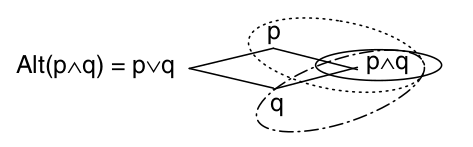
\includegraphics[width=0.33\textwidth]{ie}
    \end{center}

   \end{itemize}

    \subsection*{Application to question-answer pairs}

    \begin{itemize}

        \item As we saw earlier, we ran into the same problem of \textit{which alternatives to exclude} in cases involving question-answer pairs.

    \pex
    Who did Michael talk to?
    \a \textsc{Some} woman.\hfill \(⇝\) \textit{Michael talked to exactly one woman}
    \xe

      \item We can assume that the syntax gives us the following representation for the answer, where the set of alternatives is provided by the question (I write, e.g., $\ml{j} ∧ \ml{t}$ for $\ml{Michael talked to Janet and Tehani}$):

        \ex
        $\ml{exh}_{Q}$ [Some woman \st{Michael talked to $t$}]
        \xe

        \[
        Q = \set{p|∃ X[p = \ml{m talked to }X]}
        \]

       \item If the domain of quantification is $\set{\ml{janet},\ml{tehani},\ml{eleanor}}$, then the Hamblin set is as follows. Note that we're assuming that the alternatives are closed under disjunction -- this can be accomplished by assuming that \textit{who} ranges over atoms and pluralities; see \citealt{Dayal,fox-sub22}. More on this next time.

        \[
        \eval{who did Michael talk to?} = Q = \Set{\begin{array}{c}
            \ml{j},\ml{t},\ml{e}\\
            \ml{j} ∧ \ml{t}, \ml{j} ∧ \ml{e}, \ml{t} ∧ \ml{e}\\
            \ml{j} ∧ \ml{t} ∧ \ml{e}
          \end{array}}
        \]

      \item The maximal $p$-consistent subsets of alternatives are as follows, where $p = \ml{michael talked to some woman}$. Crucially, no maximally $p$-consistent subset contains all of the following alternatives: (a) \textit{Michael talked to Janet}, (b) \textit{Michael talked to Tehani}, (c) \textit{Michael talked to Eleanor}.

        \[
        \Set{
        \begin{array}{c}
          \set{\ml{j},\ml{t},\ml{j} ∧ \ml{t}, \ml{j} ∧ \ml{e}, \ml{t} ∧ \ml{e},\ml{j} ∧ \ml{t} ∧ \ml{e}}\\
          \set{\ml{j},\ml{e},\ml{j} ∧ \ml{t}, \ml{j} ∧ \ml{e}, \ml{t} ∧ \ml{e},\ml{j} ∧ \ml{t} ∧ \ml{e}}\\
          \set{\ml{t},\ml{e},\ml{j} ∧ \ml{t}, \ml{j} ∧ \ml{e}, \ml{t} ∧ \ml{e},\ml{j} ∧ \ml{t} ∧ \ml{e}}\\
        \end{array}
        }
        \]

      \item In order to compute the innocently excludable alternatives, we take the intersection of the maximal excludable sets of alternatives. We end up with the set of alternatives of the form $\ml{m talked to }X$, where $X$ is a plurality of women (i.e., not including atomic women!):

         \[
         \ml{IE} Q = \Set{
          \ml{j} ∧ \ml{t}, \ml{j} ∧ \ml{e}, \ml{t} ∧ \ml{e},\ml{j} ∧ \ml{t} ∧ \ml{e}
        }
        \]

      \item The result of exhaustifying \textit{Michael talked to some woman} relative to the set of innocently excludable alternatives, then, is the SI that \textit{Michael didn't talk to a plurality of women}. When conjoined with the basic meaning, this entails that Michael talked to exactly one woman. This seems correct!

        \ex
        \(\begin{aligned}[t]
          &\eval{
        $\ml{exh}_{Q}$ [Some woman \st{Michael talked to $t$}]
      }\\
      &= ∃x[\ml{woman} x ∧ \ml{m talked to }x] \begin{aligned}[t]
          &∧ ¬ (\ml{j} ∧ \ml{t})\\
          &∧ ¬ (\ml{j} ∧ \ml{e})\\
          &∧ ¬ (\ml{t} ∧ \ml{e})\\
          &∧ ¬ (\ml{j} ∧ \ml{t} ∧ \ml{e})\\
        \end{aligned}
        \end{aligned}\)
        \xe

    \end{itemize}

    \subsection*{Application to Chierchia's puzzle}

    Consider again Chierchia's puzzling example:

\pex
Eleanor did the reading or some of the homework.
\a\label{a2rep}$\not\rightsquigarrow$ \textit{Eleanor didn't do the reading or all of the homework}
\a\label{a3}$⇝$ \textit{Eleanor didn't do all of the homework}
\xe

The puzzle here is how to derive the implicature in (\ref{a3}) without also deriving the implicature in (\ref{a2rep}), without making ad-hoc assumptions about alternatives.

\begin{itemize}

    \item If we cash out alternativehood in terms of syntactic complexity, it follows that alternativehood should be \textit{transitive}. In other words, if $q ∈ \ml{alt} p$ and $q' ∈ \ml{alt} q$, then it should follow that $q' ∈ \ml{alt} p$

    \item Under this assumption, we can readily enumerate the alternatives to \textit{Eleanor did the reading or all of the homework} (which we'll abbreviate as $r∨∃h$).

    \[\ml{alt} (r∨∃h) = \Set{
    \begin{aligned}[c]
      &r∧∃h&\text{conjunctive alt}\\
      &r,∃h&\text{S-alts}\\
      &r∨∀h&\text{universal alt}\\
      &∀h&\text{S-alt of universal alt}\\
      &r ∧ ∀h&\text{conjunctive alt of S-alt}\\
      \end{aligned}
    }\]

    \item We can order these alternatives relative to truth-conditional strength:

    \begin{center}
      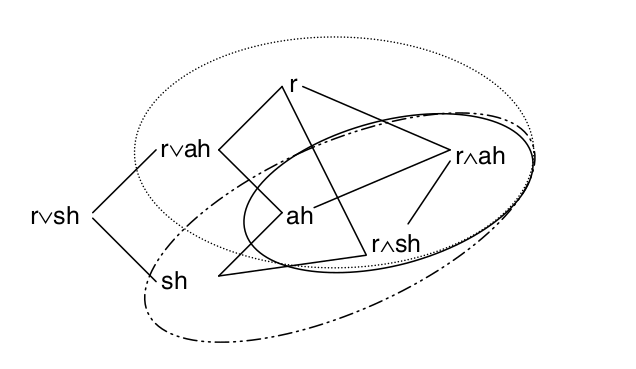
\includegraphics[width=0.3\textwidth]{ie2}
    \end{center}

  \item As illustrated in the diagram, the maximal $p$-consistent subsets of alternatives are as follows,\\
    where $p = \ml{Eleanor did the reading or some of the homework}$:

    \[
    \Set{\begin{array}{c}
           \set{r \wedge \exists h,r,r\vee \forall h, \forall h, r \wedge \forall h}\\
           \set{r \wedge \exists h,\exists h, \forall h, r \wedge \forall h}\\
          \end{array}}
    \]

  \item The intersection of the maximal $p$-consistent subsets gives us the set of innocently excludable alternatives, namely:

    \[
    \ml{IE} = \set{r ∧ ∃h, ∀ h, r ∧ ∀ h}
    \]

  \item When we exhaustify \textit{Eleanor did the reading or some of the homework} relative to the innocently excludable alternatives, we derive the following inferences:

    \begin{itemize}

      \item Eleanor did the reading or some (perhaps all) of the homework (or both).\\
        \phantom{,}\hfill basic inference

      \item Eleanor didn't do all of the homework.\hfill SI

      \item Eleanor didn't do both the reading and some or all of the homework. \hfill SI

      \item Strengthened meaning:\\
        \textit{Eleanor did either the reading, or some but not all of the homework, but not both, and she didn't do all of the homework}.

    \end{itemize}

    \item We've solved Chierchia's puzzle! For a disjunctive sentence of the form $p ∨ q$, if $q$ has a truth-conditionally stronger alternative $q'$, then $q'$ (unlike $q$) is an \textit{innocently excludable alternative} and can be negated.

\end{itemize}

\subsection*{Embedding disjunction under universal quantifiers}

\begin{itemize}

    \item There are certain environments in which conjoining a disjunctive sentence with the negations of its disjuncts \textit{doesn't} lead to a contradiction -- specifically, embedding under an upward-monotone operator $O$:

    \ex
    $O (p ∨ q) ∧ ¬ O p ∧ ¬ O q ∧ ¬ O (p ∧ q)$
    \xe

    \item I.e., if we take $O$ to be a universal modal: $p$ or $q$ are enough to fulfil the requirements, but it's not required that $p$, and it's not required that $q$, and it's not required that $p ∧ q$.

  \item What are the facts?

    \pex
    You're required to talk to Mary or Sue.
    \a $⇝$ You're not required to talk to Mary.
    \a $⇝$ You're not required to talk to Sue.
    \a $⇝$ You're not required to talk to Mary and Sue.
    \xe

    \pex
    Every friend of mine has a dog or a cat.
    \a $⇝$ Not every friend of mine has a dog.
    \a $⇝$ Not every friend of mine has a cat.
    \a $⇝$ Not every friend of mine has a cat and a dog.
    \xe

  \item Since embedding under universals allows for consistent exclusion of all the individual disjunct alternatives, so our algorithm predicts the following set of innocently excludable alternatives. In fact there is only one maximal $p$-consistent subset of alternatives.

    \begin{center}
      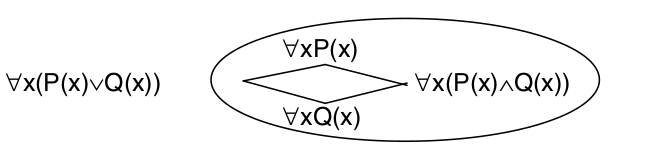
\includegraphics[width=0.3\textwidth]{ie3}
    \end{center}

    \[
    \ml{IE} = \set{∀x[P x], ∀x[Q x], ∀x[P x ∧ Q x]}
    \]

  \item Exhaustifying, e.g., \textit{every friend of mine has a dog or a cat} relative to the innocently excludable alternatives results in the following strengthened meaning:

    \[
    ∀x[P x ∨ Q x] ∧ ¬ ∀x[P x] ∧ ¬ ∀x[Q x]
    \]

\end{itemize}

\end{itemize}

\section{Recursive exhaustification and the problem of free choice}

\subsection{The problem of \textit{free choice permission}}

\pex\label{fc1}
You're allowed to eat the cake or the ice cream.
\a \textit{You're allowed to eat the cake} \hfill Free Choice inferences
\a \textit{You're allowed to eat the ice cream}
\xe

The FC inferences don't logically follow from the most obvious LF we might assign to (\ref{fc1}):

\ex
allowed [[you eat the cake] or [you eat the ice cream]]\hfill $◇ (p ∨ q)$
\xe

Assuming a possible world semantics for modality, this just means something like: \textit{there is a world consistent with the rules in which $p ∨ q$ is true}.

In fact this is equivalent to the following, which is clearly weaker than the conjunction of the FC inferences of (\ref{fc1}):

\ex
You're allowed to eat the cake or you're allowed to eat the ice cream.\hfill $◇ p ∨ ◇ q$
\xe

The abstract form of the problem is as follows:

\pex
\a $◇ (p ∨ q)$
\a $◇ p ∨ ◇ q$\hfill $a ≡ b$
\a Free Choice: $◇ p ∧ ◇ q$
\xe

\subsubsection*{Evidence that FC is a scalar implicature}

Scalar implicatures disappear in certain downward entailing environments:

\ex
Nobody talked to Michael or Janet.
\xe

\pex
\a\ljudge{*} Negation of SI: $∃ x[x \ml{talked-to-m} ∧ x \ml{talked-to-j}]$
\a Negation of standard meaning: $¬∃ x[x \ml{talked-to-m} ∨ x \ml{talked-to-j}]$
\xe

Plausibly, this is because computing the SI in such an environment results in a logically \textit{weaker} meaning: \textit{Nobody talked to Michael and not Janet, and nobody talked to Janet and not Michael, perhaps someone talked to both Michael and Janet}.

The exhaustivity operator must be subject to an economy condition, such that it isn't inserted in an LF if it weakens the global meaning of the sentence. We won't cash out exactly how to state such a condition here, but see \citet{fox_economy_2018}.

The key observation here is that, just like an SI, FC inferences disappear in certain DE environments:

\ex\label{de1}
No one is allowed to eat the cake or the ice cream.
\xe

\pex
\a\ljudge{*} negation of FC: $¬ ∃ x[◇ P x ∧ ◇ Q x]$
\a negation of standard meaning: $¬ ∃ x[◇ P x ∨ ◇ Q x]$
\xe

If the FC was indeed negated, (\ref{de1}) should be \textit{true} in a situation in which everyone is allowed to eat one of the two desserts, but nobody has free choice, i.e., in a situation where nobody is allowed to decide which dessert to eat. This seems far too weak.

If the FC inference is a SI, the logic is the same as in the basic case: the negation of the FC inferences is \textit{weaker} than the negation of the basic meaning, and therefore an economy condition on the distribution of $\ml{exh}$ rules out its insertion in such a context.

\subsection{Recursive exhaustification}

\begin{itemize}

\item Recall that ignorance inferences associated with, e.g., disjunctive sentences are computed on the basis of the MQ.

\item We've been assuming that $\ml{exh}$ can be freely prepended to any sentence. One factor which may bias towards inserting an exhaustivity operator is if it avoids otherwise undesirable ignorance inferences. Fox captures this idea with the following principle:

\ex
\textit{Recursive parsing strategy}\\
If a sentence S has an undesirable ignorance inference, parse it as $\ml{exh}$ (Alt(S)) S.
\xe

\item Consider the following:

\ex
I ate the cake or the ice cream.
\xe

\item If we decide not to insert $\ml{exh}$, and therefore not to compute any SI, the ignorance inference generated on the basis of the MQ is that \textit{speaker doesn't know what she ate}, only that it includes the cake, the ice cream, or both. Now, depending on the context, this may be an \enquote{undesirable} thing to infer (i.e., if it's common ground that the speaker knows what she ate).

\item To avoid this, we parse the disjunctive sentence with $\ml{exh}$:

\ex\label{parse}$\ml{exh} C (c \vee i)$\\
where $C = \ml{alt} (c \vee i)$
\xe

\item As we've already determined, the parse in (\ref{parse}) gives rise to the exclusive inference as an SI.

\item If we're in a context in which it's common ground that the speaker knows what she ate, this still leaves us with an undesirable ignorance inference: \textit{the speaker ate the cake or the ice cream but not both, and she doesn't know whether she ate cake, and she doesn't know whether she ate ice cream}.

\item We might try to avoid the undesirable ignorance inference by prepending $\ml{exh}$ again, in accordance with the recursive parsing strategy:

\ex\label{parse}$\ml{exh} C' (\ml{exh} C (c \vee i))$\\
where $C = \ml{alt} (\ml{exh} C (c \vee i))$
\xe

\item It turns out that recursive exhaustification has \textit{no effect}, given our algorithm for computing the strengthened meaning.

\item To see this, let's first lay out the set of alternatives to the sentence: $\ml{exh} C (c \vee i)$

    \[
    C' = \Set{
    \begin{aligned}[c]
      &\ml{exh} C (c ∨ i) &\begin{aligned}[t]
        &= (c ∨ i) ∧ ¬ (c ∧ i)\\
        &= (c ∧ ¬ i) ∨ (i ∧ ¬ c)
        \end{aligned}\\
        &\ml{exh} C c &\begin{aligned}[t]
          &= c ∧ ¬ i
          \end{aligned}\\
     &\ml{exh} C i  &\begin{aligned}[t]
          &= i ∧ ¬ c
          \end{aligned}\\
     &\ml{exh} C (c ∧ i) &\begin{aligned}[t]
          &= p ∧ q
          \end{aligned}
    \end{aligned}
    }
    \]

  \item Two things to observe here:

    \begin{itemize}

        \item The fourth alternative is already excluded by the prejacent, and hence can be ignored.

      \item The first alternative is equivalent to the disjunction of the second and the third. In other words:

        \[
        \ml{exh} C (c ∨ i) ≡ (\ml{exh} C c) ∨ (\ml{exh} C i)
        \]

    \end{itemize}

  \item The relevant alternatives are therefore $c ∧ ¬ i$  and $i ∧ ¬ c$. If the first is excluded the second must be true, and vice versa. Therefore, neither is \textit{innocently excludable}, and hence the meaning does not change with a second level of exhaustification.

    \begin{tcolorbox}
      Conclusion
      \tcblower
      In a simple disjunctive sentence, recursive application of $\ml{exh}$ doesn't change the meaning.
      \end{tcolorbox}

  \item There is no way to avoid the undesirable ignorance inference. In fact \enquote{I ate cake or ice cream} is indeed an odd thing for the speaker to utter in a context where it's common ground that she knows what she ate.

\end{itemize}

\subsection{Deriving free choice via recursive exhaustification}

\begin{itemize}

    \item Consider again the following sentence:

    \ex
    You may eat the cake or the ice cream.
    \xe

  \item According to the MQ, the following ignorance inferences are derived:

    \begin{itemize}

        \item The speaker doesn't know that you may eat cake.

      \item The speaker doesn't know that you may eat ice cream.

        \item $⇝$ the speaker doesn't know what you may eat.

    \end{itemize}

  \item Assuming we're in a context where the speaker can be assumed to be informed about what we may eat, the hearer will opt for a parse with $\ml{exh}$:

    \ex
    $\ml{exh} C $you may eat the cake or the ice cream.
    \xe

  \item i.e.:

    \[
    \ml{exh} C (◇ (c ∨ i))
    \]

    \item Assuming that the individual disjuncts count as alternatives, the set of alternatives to $◇ (c ∨ i)$ is the following (where $p ∨ q$ is subbed in for $c ∨ i$):

    \begin{center}
      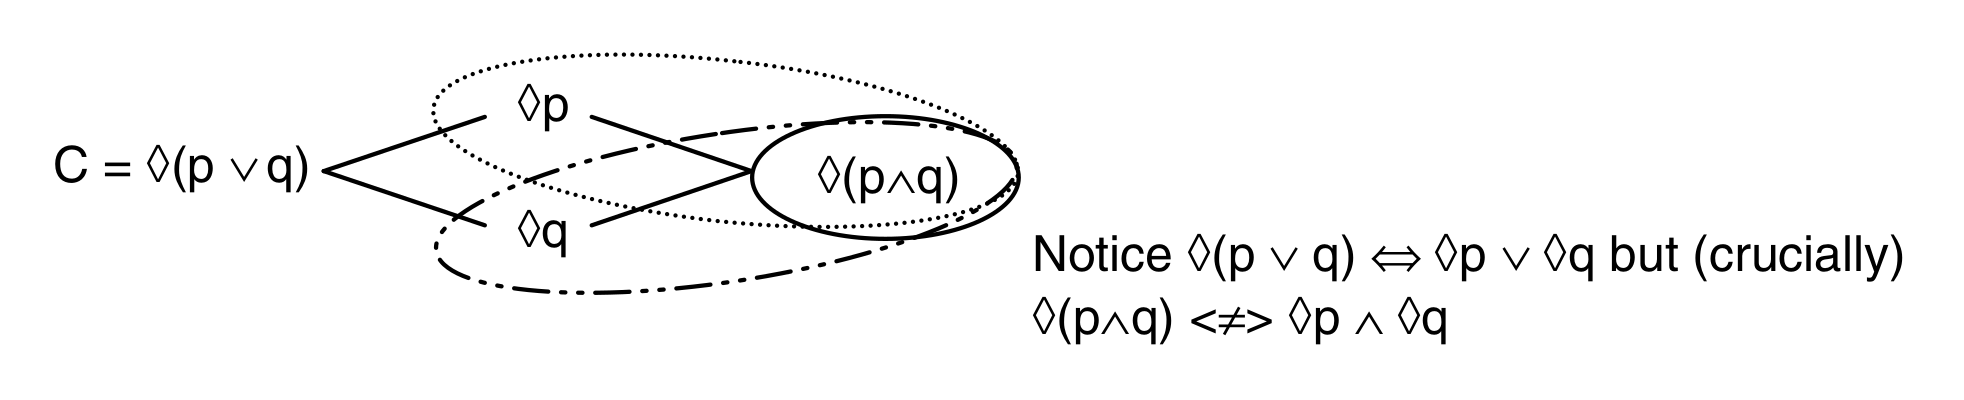
\includegraphics[width=0.5\textwidth]{ie4}
    \end{center}

  \item $◇ (c ∧ i)$ is the only proposition that may be innocently excluded, given our algorithm.

    \item The strengthened meaning is therefore:

    \[
    ◇ (c ∨ i) ∧ ¬ ◇ (c ∧ i)
    \]

    \item This is consistent with free choice possibility (i.e., $◇ c ∧ ◇ i$), but of course doesn't assert free choice.

    \item This strengthened meaning will give rise the the following ignorance inferences via MQ: \textit{the speaker doesn't know what one is allowed to eat, only that it includes cake and ice cream, but not both}.

  \item The resulting ignorance inference might be implausible, in which case we can prepend $\ml{exh}$ again:

    \ex
    $\ml{exh} C' (\ml{exh} C (◇ (c ∨ i)))$
    \xe

    \item \textit{This} time, the second exhaustification has consequences. To see this, let's first compute the meanings of the various alternatives:

    \[
    C' = \Set{
    \begin{aligned}[c]
      &\ml{exh} C (◇ (c ∨ i)) &\begin{aligned}[t]
        &= ◇ (c ∨ i) ∧ ¬ ◇ (c ∧ i)
        \end{aligned}\\
        &\ml{exh} C (◇ c) &\begin{aligned}[t]
          &= ◇ c ∧ ¬ ◇ i
          \end{aligned}\\
     &\ml{exh} C (◇ i)  &\begin{aligned}[t]
          &= ◇ i ∧ ¬ ◇ c
          \end{aligned}\\
     &\ml{exh} C (◇ (c ∧ i)) &\begin{aligned}[t]
          &= ◇ (c ∧ i)
          \end{aligned}
    \end{aligned}
    }
    \]

    \item There are now two propositions in $C'$ that can be innocently excluded, since negating $◇ c ∧ ¬ ◇ i$ does \textit{not} necessarily include $◇ i ∧ ¬ ◇ c$, and vice versa.

  \item Hence:

    \[\ml{exh} C' (\ml{exh} C (◇ (c ∨ i))) = \begin{aligned}[t]
        &◇ (c ∨ i) ∧ ¬ ◇ (c ∧ i)\\
        &∧ ¬ (◇ c ∧ ¬ ◇ i)\\
        &∧ ¬ (◇ i ∧ ¬ ◇ c)\\
        &≡ ◇ c ∧ ◇ i\\
        &∧ ¬ ◇ (c ∧ i)
      \end{aligned}\]

    \item We've derived the free choice inference for disjunction embedded under an existential modal!

\end{itemize}

\section*{Next time}

\begin{itemize}

  \item A refinement of Fox's algorithm based on \textit{universal free choice}:

    \pex
Every boy is allowed to eat ice cream or cake.
\a $⇝$ every boy is allowed to eat ice cream.
\a $⇝$ every boy is allowed to eat cake.
    \xe

    \pex~
    No student is required to solve problem A and problem B.
\a $⇝$ No student is required to solve problem A.
    \a $⇝$ No student is required to solve problem B:w
    \xe

 \item Procedure for applying \(\mathrm{EXH^{IE+II}}\) to a proposition \(p\):

\begin{itemize}
\tightlist
\item
  Negate the set of \emph{innocently excludable} members of
  \(\mathrm{Alt}(p)\).

  \begin{itemize}
  \tightlist
  \item
    To get the \emph{innocently excludable} members of
    \(\mathrm{Alt}(p)\), we gather the maximal members of
    \(𝓟(\mathrm{Alt}(p))\) that can be negated consistently with \(p\),
    and intersect them.
  \end{itemize}
\item
  Assert the set of \emph{innocently includable} members of
  \(\mathrm{Alt}(p)\).

  \begin{itemize}
  \tightlist
  \item
    To get the \emph{innocently includable} members of
    \(\mathrm{Alt}(p)\), we gather the maximal members of
    \(𝓟(\mathrm{Alt}(p))\) that can be asserted consistently with \(p\)
    and the negation of the innocently excludable alternatives, and
    intersect them.
  \end{itemize}
\end{itemize}

    \pex\label{universalFC} Every boy is allowed to eat ice cream or cake.
\hfill \(∀ x ◇(Px ∨ Qx)\)
\a \textit{Every boy is allowed to eat ice cream}. \hfill \(∀ x ◇ Px\)
\a \textit{Every boy is allowed to eat cake}. \hfill \(∀ x ◇ Qx\) \xe

\item First, let's compute the set of alternatives:

\[\begin{aligned}[t]
&\mathrm{Alt}(∀ x ◇ (Px ∨ Qx))\\
&= \Set{\begin{array}{c}
\overbrace{① ∀ x ◇ (Px ∨ Qx)}^{\text{prejacent}}, \overbrace{② ∀ x ◇ Px,③ ∀ x ◇ Qx}^{\text{universal disjunctive alts}}, \overbrace{④ ∀ x ◇ (Px ∧ Qx)}^{\text{universal conjunctive alt}}\\
\underbrace{⑤ ∃ x ◇ (Px ∨ Qx)}_{\text{existential alt}}, \underbrace{⑥ ∃ x ◇ Px,⑦ ∃ x ◇ Qx}_{\text{existential disjunctive alts}}, \underbrace{⑧ ∃ x ◇ (Px ∧ Qx) }_{\text{existential conjunctive alt}}
\end{array}}
\end{aligned}\]

\item Let's gather together the maximal subsets of
\(\mathrm{Alt}(∀ x ◇ (Px ∨ Qx))\) that can be negated consistently with
\(∀ x ◇ (Px ∨ Qx))\).

\[\Set{② ∀ x ◇ Px,③ ∀ x ◇ Qx, \alert{④ ∀ x ◇ (Px ∧ Qx)}, \alert{⑧ ∃ x ◇ (Px ∧ Qx) }}\]

\[\Set{② ∀ x ◇ Px,⑥ ∃ x ◇ Px, \alert{④ ∀ x ◇ (Px ∧ Qx)}, \alert{⑧ ∃ x ◇ (Px ∧ Qx)}}\]

\[\Set{③ ∀ x ◇ Qx,⑦ ∃ x ◇ Qx, \alert{④ ∀ x ◇ (Px ∧ qx)}, \alert{⑧ ∃ x ◇ (px ∧ qx)}}\]

    \[
\mathrm{IE}(∀ x ◇ (Px ∨ Qx)) = \Set{{④ ∀ x ◇ (Px ∧ Qx)}, {⑧ ∃ x ◇ (Px ∧ Qx)}}
\]

\item If we take the prejacent together with the negation of the IE
alternatives, we end up in a world where, either all boys are allowed to
P and not Q, all boys are allowed to Q and not P, or some boys are
allowed to P and not Q and some boys are allowed to Q and not P (no boys
are allowed to P and Q), i.e.

\[
∀ x ◇ (Px ∨ Qx) ∧ ¬ ∃ x ◇ (Px ∧ Qx)
\]

\item Let's gather together the maximal subsets of
\(\mathrm{Alt}(∀ x ◇ (Px ∨ Qx))\) that can be asserted consistently with
\(∀ x ◇ (Px ∨ Qx)) ∧ ¬ ∃ x ◇ (Px ∧ Qx)\).

\item It turns out there is only one such set, consisting of all the non-IE
alts:

\[
\Set{
\begin{array}{c}
① ∀ x ◇ (Px ∨ Qx), ② ∀ x ◇ Px,③ ∀ x ◇ Qx,\\
⑤ ∃ x ◇ (Px ∨ Qx), ⑥ ∃ x ◇ Px,⑦ ∃ x ◇ Qx
\end{array}
}
\]

\item Asserting the II alts together with the prejacent and negation of the IE
alts results in the following enriched meaning:

\[
∀ x ◇ (Px ∨ Qx) \alert{∧ ¬ ∃ x ◇ (Px ∧ Qx) ∧ ∀ x ◇ Px ∧ ∀ x ◇ Qx}
\]

\end{itemize}

\subsection{The \textit{only}-$\ml{exh}$ correspondence}

    \pex
\a \(\mathrm{EXH}^{IE}\) \alert{asserts} that its prejacent is true and
that all IE alternatives are false. \a \textit{only} \alert{presupposes}
that its prejacent is true and that all IE alternatives are false. \xe

Revised version:

\pex
\a \(\mathrm{EXH}^{IE+II}\) \alert{asserts} that all II alternatives are
true and asserts that all IE alternatives are false. \a \textit{only}
\alert{presupposes} that all II alternatives are true and that all IE
alternatives are false. \xe

\pex
We are only allowed to eat {[}ice cream or cake{]}\(_F\) \a \(⇝\) we are
allowed to eat ice cream \a \(⇝\) we are allowed to eat cake \xe

\pex
Are we only allowed to eat ice cream or cake? \a \(⇝\) We are allowed to
eat ice cream. \a \(⇝\) We are allowed to eat cake. \xe

\pex
Are we allowed to eat ice cream or cake? \a \(¬⇝\) We are allowed to eat
ice cream. \a \(¬⇝\) We are allowed to eat cake. \xe


\section{Innocent Conclusion}

\begin{itemize}

    \item The relation between exhaustification and \citeauthor{groenendijk_studies_1984}'s (\citeyear{groenendijk_studies_1984}) partition semantics.

\end{itemize}



\printbibliography

\end{document}

%%% Local Variables:
%%% mode: latex
%%% TeX-master: t
%%% End:
